\documentclass{article}

% Packages
\usepackage{algorithm}
\usepackage{algpseudocodex}
\usepackage{empheq}
\usepackage[margin=3.5cm]{geometry}
\usepackage{graphicx}
\usepackage{hyperref}
\usepackage[usestackEOL]{stackengine}

% Common commands and acronyms


\usepackage{bm}
\newcommand{\varsymbol}{q}
\newcommand{\vars}{\bm{\varsymbol}}
\newcommand{\jacobian}{\bm{J}}
\newcommand{\rhs}{\bm{F}}
\newcommand{\rhssub}[1]{\rhs(\vars_{#1})}
\newcommand{\I}{\bm{I}}
\newcommand{\dt}{\Delta t}
\newcommand{\pseudodt}{\dt^*}
\newcommand{\pseudocfl}{CFL^*}
\newcommand{\systemmat}{\bm{A}}
\newcommand{\systemmatlong}[1]{\left( \I - \dfrac{\dt}{2}\jacobian_{#1} \right)}
\newcommand{\systemmatconv}{\bm{A}_c}
\newcommand{\systemmatvisc}{\bm{A}_v}
\newcommand{\unknown}{\bm{x}}
\newcommand{\fgmres}{\texttt{FGMRES}}
\newcommand{\krylovstart}{\bm{v}}
\newcommand{\gmresprecondletter}{P}
\newcommand{\gmresprecond}{\mathcal{\gmresprecondletter}}
\newcommand{\gmrespremat}{\bm{\gmresprecondletter}}
\newcommand{\smoother}{\mathcal{S}}
\newcommand{\smootherrhs}{\bm{G}}
\newcommand{\smootherrhsconv}{\bm{G}_c}
\newcommand{\smootherrhsvisc}{\bm{G}_v}
\newcommand{\smoothervarsymbol}{u}
\newcommand{\smvec}{\bm{\smoothervarsymbol}}
\newcommand{\smprecondletter}{B}
\newcommand{\smprecond}{\mathcal{\smprecondletter}}
\newcommand{\smprecondmat}{\bm{\smprecondletter}}
\newcommand{\awmat}{\bm{W}}
\newcommand{\mgsol}{\bm{z}}
\newcommand{\mgin}{\bm{y}}
\newcommand{\mgres}{\bm{r}}
\newcommand{\restrict}{\mathcal{R}}
\newcommand{\prolong}{\restrict^{-1}}
\newcommand{\uppermat}{\bm{U}}
\newcommand{\lowermat}{\bm{L}}
\newcommand{\diag}{\bm{D}}
\newcommand{\resrhs}{\bm{b}}
\newcommand{\fluxjac}{\bm{K}}
\newcommand{\elemjac}{\mathcal{J}}
\newcommand{\elemevecr}{\mathcal{E}}
\newcommand{\elemevecl}{{{\elemevecr}^{-1}}}
\newcommand{\elemeval}{\Lambda}
\newcommand{\eigenval}{\lambda}
\newcommand{\soundspeed}{c}
\newcommand{\soundfraction}{d}
\newcommand{\smprecondsolvar}{s}
\newcommand{\smprecondsol}{\bm{\smprecondsolvar}}
\newcommand{\hcontra}[2]{h^{{#1}{#2}}}
\newcommand{\heatcapacityratio}{\gamma}
\newcommand{\pressure}{P}
\newcommand{\density}{\rho}
\newcommand{\gasconstantdry}{R_d}

\usepackage[shortcuts]{glossaries}
\usepackage{booktabs}
\makeglossaries

\glsaddkey{math}{}{\acem}{\Acem}{\acm}{\Acm}{\ACm}

\newacronym[math=\vars]{vars}{Vars}{The set of variables in the equations}
\newacronym[math=\jacobian]{jac}{Jacobian}{Derivative of the RHS w.r.t. variables $\vars$}
\newacronym[math=\rhs]{rhs}{RHS}{Right-hand side of the equations}
\newacronym[math=\I]{I}{Identity}{The identity matrix}
\newacronym[math=\dt]{dt}{dt}{The size of a (real) time step}
\newacronym[math=\pseudodt]{pseudodt}{pseudo dt}{The size of a pseudo time step}
\newacronym[math=\systemmat]{sys_mat}{Sys mat}{System to solve to move forward in time}
\newacronym[math=\unknown]{unknown}{Unknown}{The vector we are trying to solve for with $\systemmat$}
\newacronym[math=\krylovstart]{krylovstart}{Krylov 1}{Starting vector of a Krylov subspace method}
\newacronym[math=\gmresprecond]{precond}{precond}{Preconditioner in \fgmres, applies $\gmrespremat^{-1}$ to its imput}
\newacronym[math=\gmrespremat]{precondmat}{precond mat}{Preconditioner matrix for \fgmres{} ($\gmrespremat\approx\systemmat$)}
\newacronym[math=\smoother]{smoother}{Smoother}{Smoother used as part of the MG algorithm}
\newacronym[math=\mgsol]{mgout}{MG out}{Solution of a multigrid iteration}
\newacronym[math=\mgin]{mgin}{MG in}{Input vector of a MG iteration}
\newacronym[math=\mgres]{mgres}{MG res}{Residual vector (used in MG)}
\newacronym[math=\restrict]{restrict}{restrict}{Restriction operator in MG}
\newacronym[math=\prolong]{prolong}{prolong}{Prolongation operator in MG (inverse of restrict)}
\newacronym[math=\smvec]{smoothervec}{sm vec}{Variable that the smoother solves for}
\newacronym[math=\smprecond]{smprecond}{sm precond}{Preconditioner used by the smoother $\smoother$}
\newacronym[math=\smprecondmat]{smprecmat}{sm pre mat}{Matrix used by the smoother preconditioner $\smprecond$}
\newacronym[math=\awmat]{awmat}{AW mat}{Matrix that represents the implicit RK system to solve? (Additive-W)}
\newacronym[math=\uppermat]{upper}{upper}{Upper triangular part of matrix $\awmat$}
\newacronym[math=\lowermat]{lower}{lower}{Lower triangular part of matrix $\awmat$}
\newacronym[math=\diag]{diag}{diag}{Diagonal part of matrix $\awmat$}
\newacronym[math=\resrhs]{resrhs}{res RHS}{RHS of some system for which we want the residual}
\newacronym[math=\smootherrhs]{smrhs}{sm RHS}{RHS of the smoother pseudo time stepping problem}
\newacronym[math=\fluxjac]{fluxjac}{flux jac}{$5\times 5$ matrix (in 3D) of the flux jacobian in an element}
\newacronym[math=\elemjac]{elemjac}{Eq. jacobian}{Flux jacobian analytic expression for an element}
\newacronym[math=\elemevecr]{elemevecr}{Eq. evec}{Right eigenvectors analytic expression for an element}
\newacronym[math=\elemevecl]{elemevecl}{Eq. evec}{Left eigenvectors analytic expression for an element}
\newacronym[math=\elemjac]{eqjac}{Eq. jacobian}{Flux jacobian analytic expression for an element}
\newacronym[math=\elemeval]{elemeval}{Eq. eval}{Eigenvalues for an element}
\newacronym[math=c]{soundspeed}{Sound speed}{Speed of sound in m/s}
\newacronym[math=\eigenval]{eigenval}{eigenvalue}{A single eigenvalue}
\newacronym[math=\soundfraction]{soundfraction}{sound fraction}{Method parameter. Fraction of the speed of sound to use as smallest value for eigenvalues}
\newacronym[math=\smprecondsol]{smprecondsol}{sm precond sol}{Variable used as a solution to the smoother preconditioner problem}

\newacronym[]{dg}{DG}{Discontinous Galerkin}
\newacronym[]{fv}{FV}{Finite volume method/discretization}
\newacronym[]{mg}{MG}{Multigrid method}


\newglossarystyle{my}{%
  \setglossarystyle{long3colheader}%
  \renewcommand*{\glossaryheader}{%
    \toprule
    Abbr. & Symbol & Description \tabularnewline\midrule\endhead
    \bottomrule\endfoot
  }%
  \renewcommand*{\glsgroupskip}{%
     & &\tabularnewline}%
  \setlength\glsdescwidth{.08\textwidth}%
  \setlength\glspagelistwidth{.7\textwidth}%
  \renewcommand{\glossentry}[2]{%
    \glsentryitem{##1}\glstarget{##1}{\glossentryname{##1}} & $\acem{##1}$ & \glossentrydesc{##1}\tabularnewline
  }%
}

\setglossarystyle{my}

\newcommand{\todo}[1]{\textcolor{blue}{#1}}

\title{GEF}

\begin{document}
\maketitle

\section{Euler equations}

The inviscid horizontal momentum equations are ($i=1,2$):
\begin{align}
\left( \sqrt{g}\rho u^\nu u^i\right)_{,\nu} = - \sqrt{g}h^{ij}p_{,j} -2\sqrt{g} \rho \Gamma^i_{j0} u^j - \sqrt{g} \rho \Gamma^i_{jk}u^ju^k,
\end{align}

and the vertical momentum equation is written:
\begin{align}
\left(\sqrt{g}\rho u^\nu w\right)_{,\nu}=-\sqrt{g}\rho g_r-\sqrt{g} \left(\frac{\partial z}{\partial \eta}\right)^{-1} \frac{\partial p}{\partial\eta}.
\end{align}

The continuity equation takes the form
\begin{align}
\left( \sqrt{g}\rho u^\nu \right)_{,\nu} = 0.
\end{align}

The thermodynamics equation can be written in terms of virtual potential temperature $\theta_v$ has
\begin{align}
   \left( \sqrt{g}\rho \theta_v u^\nu \right)_{,\nu} = \sqrt{g} \rho \left( \frac{\theta_v}{T_v} \right) \frac{\dot{Q}}{c_{pd}}
\end{align}
where $\dot{Q}$ is the rate of heating per unit mass.

In other words, we have a variable
$\vars = \left[\begin{matrix}\rho & \rho u^1 & \rho u^2 & \rho u^3 & \rho\theta\end{matrix}\right]$
and 5 equations (please ignore the funny business with $w$ vs $u^3$):
\begin{align}
\left( \sqrt{g}\rho u^\nu \right)_{,\nu} &= 0 \\
\left( \sqrt{g}\rho u^\nu u^1\right)_{,\nu} &=
    - \sqrt{g}h^{1j}p_{,j} -2\sqrt{g} \rho \Gamma^1_{j0} u^j - \sqrt{g} \rho \Gamma^1_{jk}u^ju^k \\
\left( \sqrt{g}\rho u^\nu u^2\right)_{,\nu} &=
    - \sqrt{g}h^{2j}p_{,j} -2\sqrt{g} \rho \Gamma^2_{j0} u^j - \sqrt{g} \rho \Gamma^2_{jk}u^ju^k \\
\left(\sqrt{g}\rho u^\nu w\right)_{,\nu} &=
    -\sqrt{g}\rho g_r-\sqrt{g} \left(\frac{\partial z}{\partial \eta}\right)^{-1} \frac{\partial p}{\partial\eta} \\
\left( \sqrt{g}\rho \theta_v u^\nu \right)_{,\nu} &=
    \sqrt{g} \rho \left( \frac{\theta_v}{T_v} \right) \frac{\dot{Q}}{c_{pd}}
    \text{.}
\end{align}
$\vars$ is defined in a 4-dimensional space $X = \{x^0, x^1, x^2, x^3 \} $ where $x^0$ is
the time dimension and $x^{1-3}$ are the 3 spatial dimensions.

If we keep the time derivatives on the left and put the fluxes on the right, we get
\todo{gotta deal with $w/u^3$}
\begin{empheq}[right = \empheqrbrace\Centerstack{$:= \rhs$}]{align}
\left( \sqrt{g}\rho \right)_{,0} &= -\left( \sqrt{g}\rho u^i \right)_{,i} \\
\left( \sqrt{g}\rho u^1\right)_{,0} &=
    - \left( \sqrt{g}\rho u^i u^1\right)_{,i}
    - \sqrt{g}h^{1j}p_{,j} -2\sqrt{g} \rho \Gamma^1_{j0} u^j
    - \sqrt{g} \rho \Gamma^1_{jk}u^ju^k \\
\left( \sqrt{g}\rho u^2\right)_{,0} &=
    - \left( \sqrt{g}\rho u^i u^2\right)_{,i}
    - \sqrt{g}h^{2j}p_{,j} -2\sqrt{g} \rho \Gamma^2_{j0} u^j
    - \sqrt{g} \rho \Gamma^2_{jk}u^ju^k \\
\left(\sqrt{g}\rho w\right)_{,0} &=
    - \left(\sqrt{g}\rho u^i w\right)_{,i}
    -\sqrt{g}\rho g_r-\sqrt{g} \left(\frac{\partial z}{\partial \eta}\right)^{-1} \frac{\partial p}{\partial\eta} \\
\left( \sqrt{g}\rho \theta_v \right)_{,0} &=
    - \left( \sqrt{g}\rho \theta_v u^i \right)_{,i}
    + \sqrt{g} \rho \left( \frac{\theta_v}{T_v} \right) \frac{\dot{Q}}{c_{pd}}
    \text{.}
\end{empheq}
With $i = 1, 2, 3$, $j = 1, 2$ and $u^0 = 1$. We define $\rhs$ as the entire right-hand side
of these 5 equations.

\section{Spatial discretization}

\section{Time discretization}

What we are trying to do is advance the system in time with the following formula:
\begin{equation}\label{eq:rat2_time_step}
    \vars_{n+1} = \vars_n + \systemmatlong{n}^{-1} \dt \rhssub{n}
    \text{,}
\end{equation}
where
\begin{equation}
    \jacobian_n = \left. \dfrac{\partial\rhs}{\partial\vars} \right|_{\vars_n}
\end{equation}

From eq.~\ref{eq:rat2_time_step}, we define the system matrix $\systemmat$ as
\begin{equation}\label{eq:system_mat}
    \systemmat_n := \systemmatlong{n}
    \text{.}
\end{equation}
Multiplying both sides by $\systemmat_n$, we obtain the following linear system of
equations:
\begin{align}\label{eq:system_to_solve}
    \systemmat_n \vars_{n+1} &= \systemmat_n\vars_n + \dt \rhssub{n} \\
                             &= \resrhs
    \text{.}
\end{align}
\emph{That's what we want to do!}

After that we can simply update the new state with
\begin{equation}
    \vars_{n+1} = \vars_n + \dt\unknown_n
\end{equation}

An outline of the steps we take to solve that problem of eq.~\ref{eq:system_to_solve}:
\begin{enumerate}
    \item Use \fgmres{} as an algorithm to solve the problem (with preconditioner) (sec.~\ref{sec:fgmres})
    \item Within \fgmres, call the preconditioner on every vector in the Krylov space 
    \item In the preconditioner, convert the discretization to FV (sec.~\ref{sec:finite_volume})
    \item Call the MG algorithm on the FV vector (sec.~\ref{sec:multigrid})
    \item Within MG, use a smoother on the input of each level. The smoother solves a pseudo time stepping problem (sec.~\ref{sec:smoother})
    \item Within the smoother, use a preconditioner on the pseudo time stepping problem
\end{enumerate}


\subsection{\fgmres}\label{sec:fgmres}

Soving for $x_n$ in Eq.~\ref{eq:system_to_solve} is complicated, so we use an iterative solver, \texttt{FGMRES}.
For that, we compute the basis of a Krylov space
$$K_{basis} = \left[\begin{matrix} \krylovstart & \systemmat_n\krylovstart & \systemmat_n^2 \krylovstart & \cdots \end{matrix}\right],$$
 starting with $\krylovstart$ as the residual given by our first guess
$\krylovstart = \rhssub{n} - \systemmat_n \vars_{n+1}^{guess}$, where the guess can be just $\bm{0}$.

Since the solver converges slowly with that particular set of vector, we precondition each of them
with $\gmrespremat^{-1}$, where $\gmrespremat\approx\systemmat$.
So we get 
\begin{equation}
\tilde{K}_{basis} = \left[\begin{matrix}
    \krylovstart_0 &
    \systemmat_n\gmrespremat^{-1}\krylovstart_0 &
    \systemmat_n\gmrespremat^{-1}\krylovstart_1 & \cdots \end{matrix}\right].
    \text{.}
\end{equation}


\subsection{Conversion to finite volume}\label{sec:finite_volume}

The \fgmres{} preconditioner starts by converting the input vector into a finite volume discretization. \emph{To be completed later.}

The FV grid has the same number of nodes as the DG grid.
For a DG method with degree $N$, each DG element is subdivided into $N^d$ identical
FV elements each with one node at its centre, where $d$ is the dimension of the grid. 
The value of a field at each FV node is taken to be the value of the Lagrange 
polynomial at the same position in the corresponding DG element.
\todo{Explain in spatial discretization about Legendre polynomials}
In Fig.~\ref{fig:elem_transform_cycle}, the upper two squares show the nodal positions
and subdivision of an order-4 DG element (in 2D) into 4 FV elements.

Once converted, we use the multigrid method on the resulting FV vector.

\textbf{Note:} We are using the weak form of the discontinous Galerkin method,
which at order 1 is equivalent to a FV method, using a Rusanov solver to reconstruct interface fluxes.



\begin{figure}
    \centering
    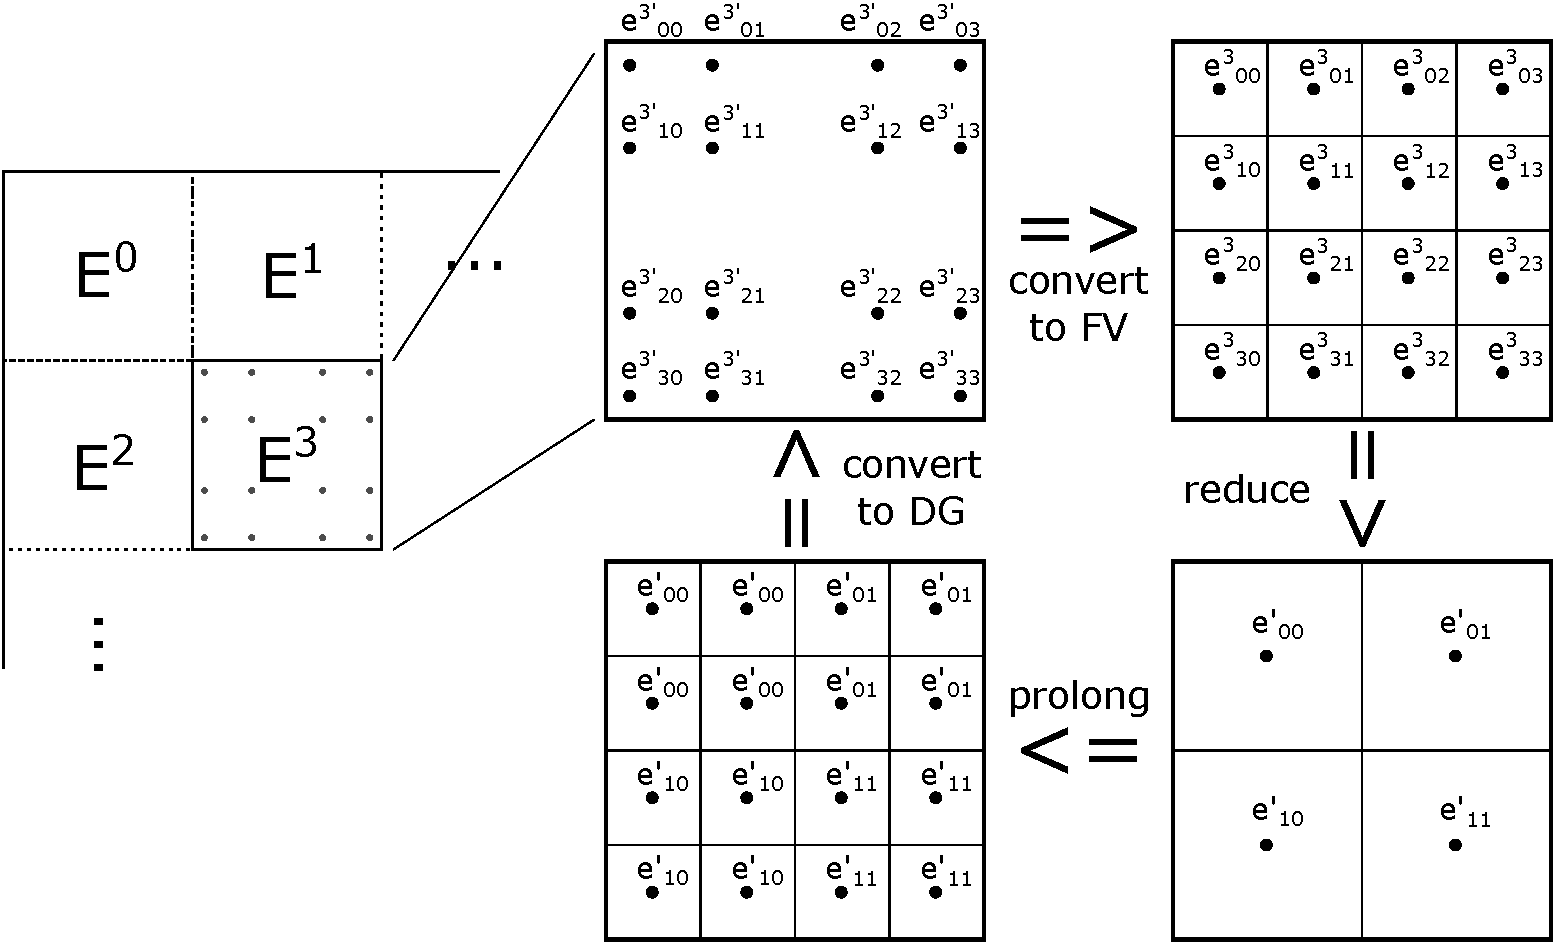
\includegraphics[width=0.8\linewidth]{img/elem_organisation}
    \caption{How the nodes of an element are transformed during a solve step.
        From upper left, going clockwise: From the DG state, we interpolate nodal
        values at the position of the FV nodes;
        from the initial FV discretization, we combine 2x2 elements (computing their 
        average value) to form a coarser grid;
        to go back to a finer grid, we set the value of each resulting element to 
        the value of its initial larger element;
        to go from FV back to DG, we use the inverse of the transformation from DG 
        to FV.
        }
    \label{fig:elem_transform_cycle}
\end{figure}

\subsection{Multigrid}\label{sec:multigrid}

Algorithm~\ref{alg:multigrid} describes our multigrid procedure.
On the first (finest) grid level, $\mgin$ is the vector to which we are applying the MG preconditioner.
On the other levels, it is the residual from the previous (finer) level.


\begin{algorithm}
    \caption{Multigrid}\label{alg:multigrid}
    \begin{algorithmic}[l]
        \State $L \gets $ number of grid levels
        \State  $\mgsol_L^0 \gets \bm{0}$ \Comment{Initial guess for $\mgsol_L$}
        \Procedure{MG}{$\mgin_l, \mgsol_l^0, l$} \Comment{On first call, $l = L$}
            \State $ \mgsol_l \gets \smoother(\systemmat_l, \mgin_l, \mgsol_l^0, \pseudodt_l) $
                    \Comment {Smoothe (0 or more times)}
            \If{$l > 0$}
                \State $ \mgres_l \gets \restrict_l (\mgin_l - \systemmat_l\mgsol_l ) $
                        \Comment{Restrict residual}
                \State $ \mgsol_{l-1} \gets \bm{0} $ \Comment{Init lower level MG}
                \For{$i = 1..\gamma$}   \Comment{Using $\gamma = 1$ all the time}
                    \State $ \mgsol_{l-1} \gets MG(\mgres_l, \mgsol_{l-1}, l - 1) $ \Comment{$\mgres_l$ = ``$\mgin$'' for next grid level}
                \EndFor
                \State $ \mgsol_l \gets \mgsol_l + \prolong_l(\mgsol_{l-1}) $ \Comment{Prolong + apply correction}
            \EndIf
            \State $ \mgsol_l \gets \smoother(\systemmat_l, \mgin_l, \mgsol_l^0, \pseudodt_l) $
                    \Comment {Smoothe (0 or more times)}
        \EndProcedure
    \end{algorithmic}
\end{algorithm}

\subsection{Smoother}\label{sec:smoother}

The smoother solves a pseudo time stepping problem 
\begin{equation}\label{eq:smoother_pseudo_time_step}
    \dfrac{\partial\smvec}{\partial t^*} = \smootherrhs(\smvec)
    \text{.}
\end{equation}
We use
\begin{equation}
    \smootherrhs(\smvec) = \resrhs - \systemmat\smvec
    \text{,}
\end{equation}
where $\resrhs$ is the vector to which we are applying the MG preconditioner (when at the finest MG grid level) and $\smvec$ is the one we are smoothing.


\subsubsection{3-stage Runge-Kutta}

We do that by using a 3-stage implicit Runge-Kutta scheme:
\begin{subequations}
\begin{align}
    \smvec^{(0)}        &= \smvec_{n} \\
    % \smvec^{(i)}        &= \smvec_{n} + \alpha_i\pseudodt\smprecondmat^{-1}\smootherrhs^{(i-1)}
    \smvec^{(i)}        &= \smvec_{n} + \alpha_i\pseudodt\smootherrhs^{(i-1)}
            \label{eq:smoother_with_precond} \\
    \smootherrhs^{(i)}  &= \smootherrhs(\smvec^{(i)}) \\
    \smvec_{n+1}        &= \smvec^{(3)} & \leftarrow \text{ the output}
\end{align}
\end{subequations}

% where $\smprecondmat$ approximates the approximation $\awmat$ of the jacobian of the implicit system
% \todo{that we should detail at eq.~\ref{eq:smoother_pseudo_time_step}}.

% \begin{align}
%     \smprecondmat &\approx \awmat
% \end{align}
% and
% \begin{align}
%     \awmat        &\approx \I + \eta\pseudodt\systemmat
% \end{align}
% where $\eta$ is a parameter.

\subsubsection{Additive Runge-Kutta}

We split the smoother problem into two portions:
\begin{equation}
    \smootherrhs(\smvec) = \smootherrhsconv(\smvec) + \smootherrhsvisc(\smvec)
    \texttt{,}
\end{equation}
with
\begin{align}
    \smootherrhsconv(\smvec) &= \resrhs - \systemmatconv\smvec \\
    \smootherrhsvisc(\smvec) &= -\systemmatvisc\smvec
    \texttt{,}
\end{align}
and use a different set of parameters for each of these portions.
The smoother becomes:
\begin{subequations}
\begin{align}
    \smvec^{(0)}        &= \smvec_{n} \\
    \smvec^{(i)}        &= \smvec_{n} + \alpha_i\pseudodt(\smootherrhsconv^{(i-1)} + \smootherrhsvisc^{(i-1)})  \\
    \smvec_{n+1}        &= \smvec^{(3)} & \leftarrow \text{ the output}\\
    \smootherrhsconv^{(i)} &= \smootherrhsconv(\smvec^{(i)}) \\
    \smootherrhsvisc^{(0)} &= \smootherrhsvisc(\smvec^{(0)}) \\
    \smootherrhsvisc^{(i)} &= \beta_i\smootherrhsvisc(\smvec^{(i)}) + (1 - \beta_i) \smootherrhsvisc^{(i-1)}
\end{align}
\end{subequations}

\subsubsection{Smoother parameters}

For the alpha and beta parameters, we take
\begin{align}
    \alpha &= \left[\begin{matrix} 0.145 & 0.395 & 1.0 \end{matrix}\right] 
    & \todo{\text{should try }\left[\begin{matrix} 0.1481 & 0.4 & 1.0 \end{matrix}\right]}\\
    \beta  &= \left[\begin{matrix} 1.0 & 0.5 & 0.5 \end{matrix}\right]
\end{align}

For the pseudo time step:
\begin{equation}
    \pseudodt = \dfrac{min(\Delta) \cdot f \cdot \pseudocfl}{max(v^i) \cdot \dt}
    \text{.}
\end{equation}
Where
\begin{itemize}
\item $min(\Delta)$ is the minimum distance between two grid points in 
    standard element coordinates ($[-1, 1]$).
\item $f = \dfrac{1}{ndim \left(2\cdot order + 1\right)}$ is a factor that's been here for a while,
    proportional to the discretization order and dimension.
\item $\pseudocfl$ is a multiplicative parameter used to adjust the pseudo time step $\pseudodt$.
    That's the one we have to specify when launching a simulation
\item $\dt$ is the time step size (in seconds) of the problem we're simulating.
\item $max(v^i)$ is the maximum speed along any of the three axes (in either direction),
    with $v^i$ the absolute value of the velocity along axis $i$:
    \begin{equation}
        v^i = \soundspeed \sqrt{\hcontra{i}{i}} + \left|u^i\right|
        \text{,}
    \end{equation}
    with $c$ the speed of sound, $u^i$ the fluid velocity along direction $i$ and $\hcontra{x}{y}$
    the contravariant metric tensor. $u^i$ is in standard element coordinates.
    $\soundspeed$ is computed as
    \begin{equation}
        c = \sqrt{\dfrac{\heatcapacityratio\pressure}{\density}}
        \text{,}
    \end{equation}
    where $\heatcapacityratio$ it the heat capacity ratio for dry air (a constant parameter),
    $\pressure$ is the pressure
    \begin{equation}
        \pressure = \pressure_0 \left(\dfrac{\gasconstantdry}{\pressure_0}\density\theta\right)^\heatcapacityratio
        \text{,}
    \end{equation}
    with $\pressure_0$ the reference pressure (constant) and $\gasconstantdry$ the gas constant for dry air.
    $\soundspeed$ is multiplied by the contravariant tensor to convert it to the same coordinates
    as the velocity $u$.
    \emph{Note: Pretty sure the computation for $\soundspeed$ is correct because the result is usually
    between 300 and 350.
    Also, when multiplied by $\hcontra{}{}$ it's about 10-30 times larger than $u$, which makes sense.}
\end{itemize}


\appendix

\section{More detailed equations}

With some identity, the equations become (only u1, u2 and u3 equations are different):
\begin{align}
\left( \sqrt{g}\rho u^\nu \right)_{,\nu} &= 0 \\
\label{eq:euler_u1}
\frac{\partial}{\partial t}\left( \sqrt{g}\rho u^1\right) 
        + \frac{\partial}{\partial x^j}\left( \sqrt{g}\left[\rho u^1u^j+h^{1j}p\right]\right)
    &= -2\sqrt{g} \, \Gamma^1_{j0} \rho u^j - \sqrt{g} \, \Gamma^1_{jk}\left(\rho u^ju^k+h^{jk}p\right) \\
\label{eq:euler_u2}
\frac{\partial}{\partial t}\left( \sqrt{g}\rho u^2\right)
        + \frac{\partial}{\partial x^j}\left( \sqrt{g}\left[\rho u^2u^j+h^{2j}p\right]\right)
    &= -2\sqrt{g} \, \Gamma^2_{j0} \rho u^j - \sqrt{g} \, \Gamma^2_{jk}\left(\rho u^ju^k+h^{jk}p\right) \\
\label{eq:euler_u3}
\frac{\partial}{\partial t}\left( \sqrt{g}\rho u^3\right)
        + \frac{\partial}{\partial x^j}\left( \sqrt{g}\left[\rho u^3 u^j + h^{3j}p\right]\right)
    &= - \sqrt{g} \rho \left(\frac{\partial z}{\partial \eta}\right)^{-1}
    g_r -2\sqrt{g} \, \Gamma^3_{j0} \rho u^j - \sqrt{g} \, \Gamma^3_{jk}\left(\rho u^ju^k+h^{jk}p\right) \\
\left( \sqrt{g}\rho \theta_v u^\nu \right)_{,\nu}
    &= \sqrt{g} \rho \left( \frac{\theta_v}{T_v} \right) \frac{\dot{Q}}{c_{pd}}
    \text{.}
\end{align}

Expanding on all of these, the flux derivatives (spatial derivatives on the LHS) are
\begin{align}
        \frac{\partial}{\partial x^1}\left( \sqrt{g}\rho u^1 \right)
      + \frac{\partial}{\partial x^2}\left( \sqrt{g}\rho u^2 \right)
      + \frac{\partial}{\partial x^3}\left( \sqrt{g}\rho u^3 \right) \\
        \frac{\partial}{\partial x^1}\left( \sqrt{g}\left[\rho u^1u^1+h^{11}p\right]\right)
      + \frac{\partial}{\partial x^2}\left( \sqrt{g}\left[\rho u^1u^2+h^{12}p\right]\right)
      + \frac{\partial}{\partial x^3}\left( \sqrt{g}\left[\rho u^1u^3+h^{13}p\right]\right) \\
        \frac{\partial}{\partial x^1}\left( \sqrt{g}\left[\rho u^2u^1+h^{21}p\right]\right)
      + \frac{\partial}{\partial x^2}\left( \sqrt{g}\left[\rho u^2u^2+h^{22}p\right]\right)
      + \frac{\partial}{\partial x^3}\left( \sqrt{g}\left[\rho u^2u^3+h^{23}p\right]\right) \\
        \frac{\partial}{\partial x^1}\left( \sqrt{g}\left[\rho u^3u^1+h^{31}p\right]\right)
      + \frac{\partial}{\partial x^2}\left( \sqrt{g}\left[\rho u^3u^2+h^{32}p\right]\right)
      + \frac{\partial}{\partial x^3}\left( \sqrt{g}\left[\rho u^3u^3+h^{33}p\right]\right) \\
        \frac{\partial}{\partial x^1}\left( \sqrt{g}\rho\theta_v u^1 \right)
      + \frac{\partial}{\partial x^2}\left( \sqrt{g}\rho\theta_v u^2 \right)
      + \frac{\partial}{\partial x^3}\left( \sqrt{g}\rho\theta_v u^3 \right)
\end{align}

\section{Lagrange polynomial interpolation from DG to FV}

In 1 dimension, the value of a field at position $x$ inside a DG element of order $N$
is defined as
\begin{equation}
    L(x) = \sum_1^N e_i l_i(x)
    \text{,}
\end{equation}
where $e_i$ is the value of field at node $i$ of the element, and $l_i$ is the $i^{th}$ basis of
the Lagrange polynomial.
In 2 dimensions, we can interpolate in 

Since each dimension of a reference element is identical, 

\glsaddallunused
\printglossaries
\end{document}
